\documentclass[a4paper,12pt,reqno]{amsart}
\usepackage{M67tds}
\usepackage{cancel}



% pour voir les solutions il faut enlever le commentaire de la ligne suivante
\solutionstrue

% Les notes de bas de page sont des symboles
\renewcommand{\thefootnote}{\fnsymbol{footnote}}

% pour surligner
\sisolutions{
  \usepackage{soul}
  \colorlet{hl}{yellow!35!white}
  \sethlcolor{hl}
  \newcommand*{\hlm}[1]{\colorbox{hl}{$#1$}}
  \newcommand*{\hldm}[1]{\colorbox{hl}{$\displaystyle #1$}}
}

\begin{document}

% ==================================
\hautdepage{

\ifsolutions{Solutions de l'interrogation}\else{Interrogation}\fi\par\normalfont\normalsize
9 avril 2018\\{[ durée: 1 heure ]}\par
}
% ==================================
\ifsolutions\else
% {\fontencoding{U}\fontfamily{futs}\selectfont\char 66\relax}
\tikz[baseline=(e.base)]{\NoAutoSpacing\node(e){!};\draw[red,ultra thick,line join=round,yshift=-.15ex](90:1em)--(210:1em)--(330:1em)--cycle;}
\textbf{Documents autorisés :}\textit{Une feuille A4 recto-verso écrite à la main.}

\vspace{21mm}
\fi


%-----------------------------------
\begin{exo} (Carré dans un  triangle)

  Soient $\tri ABC$ un triangle, $H$ le pied de la hauteur issue de $A$, et $IJKL$ un carré tel que $I \in [AB]$, $J,K \in [BC]$ et $L \in [CA]$. On note les longueurs $a=BC$ , $h=AH$ et $d=IJ$.
  \begin{enumerate}
    \item Déterminer une relation entre les longueurs $a$ , $h$ et $d$.\\
    \begin{indication}
      Vous pouvez utiliser Thalès à deux reprises.
    \end{indication}
    \item Exprimer le rapport des aires du carré $IJKL$ et du triangle $\tri ABC$ en fonction de $a$ et~$h$.
    \item Que vaut ce rapport dans le cas où le triangle $\tri ABC$ est équilatéral ?
  \end{enumerate}
\end{exo}

\begin{solution}
  \begin{enumerate}
    \item
      D'après Thalès appliqué à $[IL]//[BC]$ on a $\frac{d}{a} = \frac{AI}{AB}$.
      \sidebyside{.7}{
        D'après Thalès appliqué à $[IJ]//[AH]$ on a $\frac{d}{h} = \frac{BI}{BA}$.\\
        Et comme $\frac{AI}{AB}+\frac{BI}{BA}=\frac{AI+IB}{AB}=1$ on trouve
        \begin{center}
          \hldm{\frac{d}{a}+\frac{d}{h}=1}.
        \end{center}
      }{
        \raisebox{-11mm}[0pt][0pt]{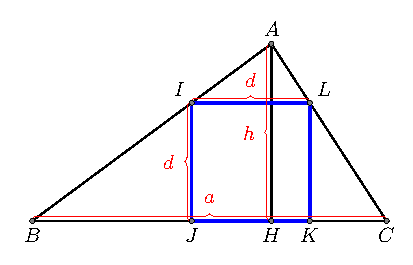
\includegraphics[width=5cm]{M67_2017-18_CC_img_triangle}}
      }
    \item D'après la question précédente $dh+da=ah \implies d=\frac{ah}{a+h}$. Ainsi le rapport des aires est
      \begin{center}
        \hldm{\mathcal{A}_{IJKL}:\mathcal{A}_{\tri ABC}}
          $=\left(\frac{ah}{a+h}\right)^{2}:\frac{ah}{2}$
          \hldm{=\frac{2ah}{(a+h)^2}}.
      \end{center}
    \item Dans le triangle équilatéral $\tri ABC$ on a la relation $h=\frac{\sqrt{3}}{2}a$ et donc
      \begin{center}
        \hldm{\mathcal{A}_{IJKL}:\mathcal{A}_{\tri ABC}}
          $= \frac{2\cancel{a^2}\frac{\sqrt{3}}{2}}{\cancel{a^2}(1+\frac{\sqrt{3}}{2})^2}=\frac{4\sqrt{3}}{7+4\sqrt{3}}$
        \hldm{=4(7\sqrt{3}-12)}\footnote{$4(7\sqrt{3}-12)\approx\frac{1}{2}$}.
      \end{center}
  \end{enumerate}
\end{solution}

\sisolutions{\tsvp\newpage}

%-----------------------------------
\begin{exo} (cas particulier du théorème de Ptolémée)

  Soient $\tri ABC$ un triangle équilatéral et $M$ un point du cercle circonscrit situé sur le petit arc $\stackrel{\frown}{BC}$ (qui ne contient pas $A$). Montrer l'égalité
  $$
    MA = MB+MC.
  $$
  \ifsolutions
    \vspace{-1cm}
  \else
    \emph{
      Plusieurs démarches sont possibles:
      \begin{itemize}
        \item en utilisant la trigonométrie, et l'expression de la longueur d'une corde;
        \item en utilisant la construction vue en td pour la démonstration du théorème de Ptolémée, qui introduit un point $K$ sur $[AM]$;
        \item en comparant des surfaces.
      \end{itemize}
    }
  \fi
\end{exo}

\begin{solution}

  \textbf{Méthode 1} \emph{(utilisant la trigonométrie)}

  \sidebyside{.7}{
    Soit $2\theta$ la mesure du petit arc $\stackrel{\frown}{MB}$, donc $(120°-2\theta)$ et $(120°+2\theta)$ sont les mesures respectivement de $\stackrel{\frown}{CM}$ et $\stackrel{\frown}{AM}$. En utilisant le fait que la longueur d'une corde d'arc $2\gamma$ est $D\sin(\gamma)$, où $D$ est le diamètre du cercle, on trouve $MA = D\sin(60°+\theta)$, $MB = D\sin(\theta)$ et $MC = D\sin(60°-\theta)$. Donc on a l'équivalence
  }
  {
    \raisebox{-28mm}[0pt][0pt]{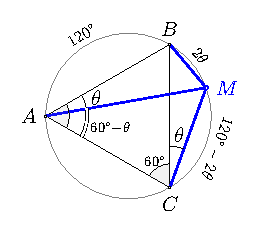
\includegraphics[width=5cm]{M67_2017-18_CC_img_trigo}}
  }
  \begin{center}
    \hldm{MA = MB + MC \;\iff\;  \sin(60°+\theta) = \sin(\theta)+\sin(60°-\theta)}.
  \end{center}
  On peut démontrer cette deuxième égalité par des méthodes différentes, par exemple en utilisant la formule $\sin(\alpha+\beta) = \sin(\alpha) \cos(\beta) + \cos(\alpha)\sin(\beta)$ on trouve
  \begin{align*}
    \sin(60°+\theta) &= \sin(60°) \cos(\theta) + \cos(60°)\sin(\theta)  \\
    \sin(\theta)+\sin(60°-\theta) &= \sin(\theta) + \sin(60°) \cos(\theta) - \cos(60°)\sin(\theta)
  \end{align*}
  et comme $1-\cos(60°)=\cos(60°)$ on obtient l'égalité cherchée.

  \textbf{Méthode 2} \emph{(par construction géométrique)}

  Nous allons utiliser ici la même construction géométrique que celle vue en td pour le théorème de Ptolémée.
  \sidebyside{.7}{
    Soit $K$ un point sur $[AM]$ tel que $MK=MB$. Comme $\widehat{BMA} = \widehat{BCA} = 60°$, le triangle $\tri BMK$ est équilatéral. Ainsi la rotation à $60°$ autour de $B$ envoie $A$ en $C$ et $K$ en $M$, donc $KA=MC$.
    On conclut avec $MA = MK+KA = MB+MC$.\\
  }{
    \raisebox{-28mm}[0pt][0pt]{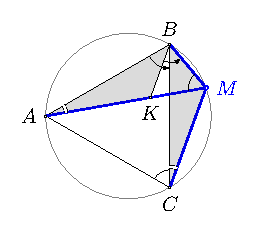
\includegraphics[width=5cm]{M67_2017-18_CC_img_ptolemee}}
  }
\end{solution}

\end{document}
